% !TEX TS-program = pdflatex
% !TEX encoding = UTF-8 Unicode

\documentclass[11pt]{article}

\usepackage[utf8]{inputenc}

%%% PAGE DIMENSIONS
\usepackage{geometry}
\geometry{a4paper} 
\geometry{margin=1in}
%   read geometry.pdf for detailed page layout information

\usepackage{graphicx} % support the \includegraphics command and options

\usepackage[parfill]{parskip} % Activate to begin paragraphs with an empty line rather than an indent

%%% PACKAGES
\usepackage{booktabs} % for much better looking tables
\usepackage{array} % for better arrays (eg matrices) in maths
\usepackage{paralist} % very flexible & customisable lists (eg. enumerate/itemize, etc.)
\usepackage{verbatim} % adds environment for commenting out blocks of text & for better verbatim
\usepackage{subfig} % make it possible to include more than one captioned figure/table in a single float
\usepackage{float}


%%% HEADERS & FOOTERS
\usepackage{fancyhdr} 
\pagestyle{fancy} 
\renewcommand{\headrulewidth}{0pt} 
\lhead{}\chead{}\rhead{}
\lfoot{}\cfoot{\thepage}\rfoot{}

%%% SECTION TITLE APPEARANCE
\usepackage{sectsty}
% \allsectionsfont{\sffamily\mdseries\upshape} % (See the fntguide.pdf for font help)
% (This matches ConTeXt defaults)

%%% ToC (table of contents) APPEARANCE
\usepackage[nottoc,notlof,notlot]{tocbibind} % Put the bibliography in the ToC
\usepackage[titles,subfigure]{tocloft} % Alter the style of the Table of Contents
\renewcommand{\cftsecfont}{\rmfamily\mdseries\upshape}
\renewcommand{\cftsecpagefont}{\rmfamily\mdseries\upshape} % No bold!
\setcounter{secnumdepth}{0}


\title{Building a database on S3? That is the title of the article.}
\author{Odd M. Trondrud}
\date{November 2013} % Activate to display a given date or no date (if empty),
         % otherwise the current date is printed 

\begin{document}
\maketitle

\begin{abstract}
A report about the article ``Building a database on S3.''
It presents a brief summary of the article and briefly discusses security and client management concerns with the implementation proposed by the article.
Reasons for why one might to do such a thing as build a database on top of S3 are discussed at the end.
\end{abstract}


\section{Introduction}
\textit{``Imagine, if you will, a worry-free world.''}
% This is supposed to be a quote but \quote didn't really do the trick, visually speaking.

Traditional system administration involved maintaining the system's hardware as well as everything else.
Some enjoy this while others would rather not crawl around in tight spaces and tinker with something physical in addition to their other duties.
And assystems grow more complex and fields expand outwards, being a jack-of-all trades becomes an unsustainable venture for the individual.
Will society progress towards a future in which each individual must specialize so thoroughly in one field that their usefulness in all other fields diminish to nothing?
Who knows.

Either way, service providers (like those guys who started selling books on the internet) have figured out how to turn a profit by providing certain services at a sufficiently large scale.
Take their Simple Storage System, for example:
A near infinitely scalable and concurrent file storage service (for the consumers).
If the availability drops below $99.9\%$ the customers receive a discount.
Such a service is typically referred to as a ``cloud'' or ``utility'' service.
Possibly because there's always a cloud somewhere on this planet and iif all clouds were connected to the internet and stored the same information with a promise of \textit{eventual concurrency} you'd be able to reach your information from wherever.

If one were to maintain such a system one would require a minimum of the maximum expected storage space for the system's data, and then enough extra storage for backups and mirroring in case of disk failures.
One would have to pay for an internet connection capable of handling a way higher load than what's expected.
And people would have to be kept on payroll to maintain the physical parts of the system as well as the non-physical parts like the software.
To summarise it is a load of hassle.

However there exists \textit{utility service providers} that provide for their customers such a service and run a by-use payment model.
In other words, the customers' infrastructure becomes near infintely scalable and concurrent without the customer having to pay the overhead such an infrastructure would impose on them if they were to develop and maintain it themselves.
Ah, the future! Isn't it great?

The article, ``Building a database on S3'', lays down an outline of how one could build a near infinitely scalable database system on top of Amazon's Simple Storage Service (S3).
The proposed system exploits the high level of availability Amazon offers with its S3\footnote{$99.9\%$ uptime as of November 2013}

\section{The Proposed Implementation}
\begin{figure}[H]
	\begin{center}
		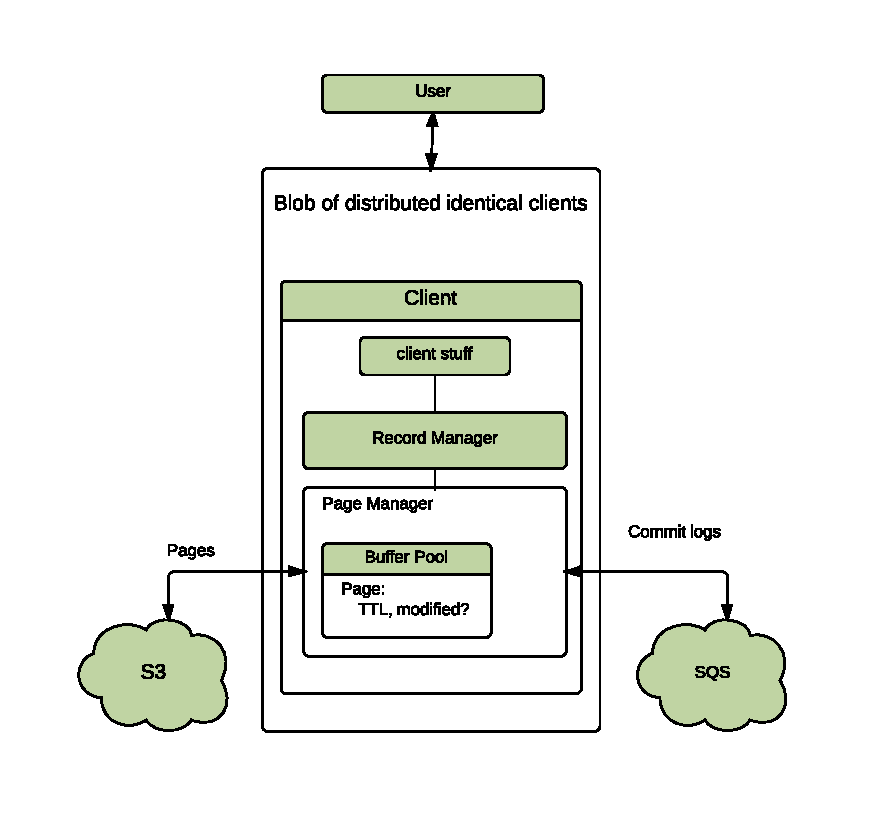
\includegraphics{img/proposed-architecture.pdf}
		\caption{An overview of the suggested architecture in the article.}
		\label{figure:proposed-architecture}
	\end{center}
\end{figure}

\section{Scalability and bottlenecks}
While the article claims that the proposed implementation would be able to support a very large number of concurrent clients, effectively eliminating the DBMS as a potential bottleneck, it does not discuss how the number of clients could be managed.
An ideal scalable system should scale itself automatically, the number of active clients at any given time, growing and shrinking with the number of active users.
A ``master'' client that monitors traffic and load on the system and spawns and terminates clients as needed could be introduced, however this could result in the master client becoming a new bottleneck.
Alternatively each client could be allowed to spawn new clients whenever the load passes over some threshold and diverting traffic to other clients (new clients could be given a copy of the spawning client's buffer pool to reduce the amount of requests to S3).
Clients could terminate themselves when the load passes below some threshold, however if there is only one active client it should not be allowed to terminate itself.
This introduces the question of how traffic should be diverted between clients, which depends on the application's nature.
Research has probably been done on this and could be worth looking into.


\section{Security}
The article barely touches on security concerns related to such a truly distributed system which it proposes.
It states that read and/or write privileges to a collection (i.e. a \textit{bucket} in S3 terminology) can be restricted on a per-client basis by the client that owns the collection, and that a security infrastructure \textit{can} be implemented on top of S3 however it does not present an explanation of \textit{how}.
This is somewhat understandable as the definition of ``client'' provided by the article\footnote{"\[\dots\] refer to software artifacts that retrieve pages from S3 and write pages back to S3."} is rather vague and implementing a proper security infrastructure for a system one knows very little about can be difficult.

However, guesstimation is possible and there are certain general security-related issues that arise when dealing with distributed systems.

\subsection{Data Encryption}
If your data is proper sensitive like you probably shouldn't store it on a service you don't control.
However, just because 

However, from examining what security features Amazon now\footnote{November 2013} offers along with its SQS and S3 services it is possible to deduce with what kind of system a certain level of security is possible to achieve.



\subsection{Data Encryption}
Amazon offers Server-Side Encryption of data stored on S3.
However one should not trust others to keep one's own secrets.
Wholly relying on the offered Server-Side Encryption means that data arrives at Amazon's data centres unencrypted.
Regardless of how much trust one places in the service provider, this approach renders the system vulnerable to a man in the middle attack. 

Client-Side Encryption is possible as objects in S3 are simply byte streams with some S3 metadata (such as the object's URI).
The metadata does not contain any information about the object's contents, so it can be left unencrypted.
The actual data however, should be encrypted on the client-side 
Performing Client-Side Encryption increases the complexity of the task of obtaining the data.
It also increases the complexity of the system as each client would have to be able to decrypt the data.


would require that an attacker is also in posession of the private key used to encrypt the data 

since some authentication scheme is required on the clients it is not advisable to allow the users physical or root access to the machines on which the client runs. In other words, the clients should rather be running on servers and users should interface with the clients over the magic that is the internet.

S3 a
If unencrypted data travels thr
is at some point outside of a controlled closed system 
If data arrives at Amazon's centres unencrypted 
However, if your data is unencrypted as it arrives Amazon's 

Client-Side Encryption would require that all involved clients 

\subsection{Client Authentication}
Some sort of client authentication would be advisable to make it harder for attackers to overwrite all your data with rubbish.



Oooh also load balancing is a question the article doesn't discuss nor how to 

\section{Eventual Consistency}
Messages can be retained in SQS for up to 14 days.

\section{How bad is the eventual consistency?}
We don't know! The article didn't test it.

\subsection{A subsection}

More text.

%% Summary
Would one want to build a database on S3?
Well, there's nothing wrong with that kind of scalability but it depends on what the bottleneck of your web service is going to be.
If your service, for some reason, is incompatible with any sort of caching or if it's built around users somehow submitting information to be stored in the database then... maybe?
One should price shop: look at alternatives (to both infrastructure and the service's structure).

When developing a service one should try and think about such things as ``what is the maximum amount of users this service needs to be able to serve at once?'' and ``what kind of traffic/activity is the average user going to generate?'' and ``how high does the service's availability need to be?''.
There'll probably be questions or cases that are more specific to particular services, but unless the answer to these three questions are ``infinity'', ``all of it'' and ``$99.\bar{o}\%$'' then the service probably does not need all that ``building a database on S3'' (or similar solutions, like SimpleDB) offers.
However it does help, but there's probably alternatives out there to building a database on S3 and \textit{you should try and look for them}.

\end{document}
